\chapter{结合自动属性提示与自训练知识蒸馏的零样本细胞核检测}

本章在第三章基于 GLIP 的零样本细胞核检测研究基础上，进一步研究如何自动构造更适合病理图像的文本提示，以及如何利用初始零样本预测缓解密集细胞核场景下的漏检和目标重叠问题。本章方法来源于论文 \emph{AttriPrompter: Auto-Prompting with Attribute Semantics for Zero-shot Nuclei Detection via Visual-Language Pre-trained Models}，是第三章工作的扩展版本。与第三章侧重于建立零样本检测流程不同，本章重点分析提示语义粒度、提示序列顺序和知识蒸馏对检测性能的影响，并给出更系统的跨域实验。

需要特别说明的是，本章所说的“零样本”是指不使用目标测试集的人工检测标注进行训练；方法仍然可以使用目标域的无标注训练图像完成属性生成、提示筛选和伪标签自训练。因此，本章也将其称为“无标注零样本检测”或“标签免除的目标域适配”，以区分完全不接触目标域图像的严格零样本设定。

\section{研究背景与问题提出}

在数字病理分析中，细胞核检测是细胞计数、空间组织学分析、肿瘤分级和预后评估等任务的重要基础。对于 H\&E 染色病理图像，细胞核通常数量多、分布密集且相互接触。同一视野内的细胞核在颜色、形状和纹理上具有较强相似性，导致检测器容易出现漏检、误检以及相邻细胞核被合并的问题。虽然全监督检测和实例分割方法在多个数据集上取得了较好结果，但其训练依赖大量逐实例标注，而病理图像标注通常需要专业人员参与，具有成本高、耗时长和主观误差明显等特点。

为降低标注依赖，已有研究从弱监督、自监督和无监督学习等方向开展探索。弱监督方法可以使用点标注或图像级标注，但这些标注仍然需要人工制作；无监督方法则往往通过阈值、尺寸、尺度或域适配假设构造训练信号，方法性能容易受到经验性规则的影响。对于密集细胞核检测而言，如何在不使用检测标注的情况下获得可靠的初始定位，仍然是一个具有挑战性的问题。

视觉语言预训练模型（Visual-Language Pre-trained Models，VLPMs）从大规模图文对中学习视觉和文本之间的对应关系，在开放词汇识别和零样本目标检测中表现出较强的迁移能力。Grounded Language-Image Pre-training（GLIP）进一步利用短语定位数据和目标级跨模态交互，获得了比一般图像级视觉语言模型更强的目标级表示能力。然而，GLIP 的预训练数据主要来自互联网自然图像，医学图像中的细胞核概念、染色特征和密集排列模式在其语义空间中覆盖不足。直接把 ``nuclei'' 作为文本提示，往往不能稳定地激活与细胞核对应的目标级视觉表示。

因此，本章围绕两个问题展开研究：第一，能否从无标注病理图像中自动发现能够描述细胞核的属性，并将这些属性组织成适合 GLIP 的文本提示；第二，能否利用 GLIP 的初始预测作为伪标签，在不遗忘其通用目标级知识的前提下，训练更适合密集细胞核检测的学生网络。针对这两个问题，本章提出自动属性提示框架 AttriPrompter，并进一步提出自训练知识蒸馏（Self-trained Knowledge Distillation，SKD）框架。

本章的主要工作包括：
\begin{itemize}
  \item 通过提示实证分析揭示语义描述粒度和提示序列顺序对 GLIP 零样本检测的影响，说明程度属性和相关性排序对细胞核定位的重要作用。
  \item 提出 AttriPrompter 自动提示框架，利用 GLIP 和 BLIP 从无标注图像中生成形状、颜色属性，并通过同义增强、程度增强和相关性排序形成最终提示序列。
  \item 提出 SKD 框架，以 GLIP 作为教师网络，以 AttriPrompter 产生的预测作为初始伪标签，通过检测损失和特征蒸馏损失训练学生网络，并采用多轮自训练不断更新伪标签。
  \item 在 MoNuSeg 和 CoNSeP 数据集上开展对比、消融、伪标签质量、学生网络结构和跨域实验，分析各组成部分的作用及方法的适用边界。
\end{itemize}

\section{视觉语言预训练与 GLIP 基础}

视觉语言预训练模型通常从大规模图文对 $\{(x_i,t_i)\}_{i=1}^{K}$ 中学习视觉表示和文本表示之间的对应关系。设图像编码器和文本编码器分别为 $E_{\mathcal V}$ 与 $E_{\mathcal T}$，一种典型的图文对比学习目标可以写为：
\begin{equation}
\label{eq:attrip_contrastive}
\mathcal{L}_{c}=-\sum_{i=1}^{K}\log
\frac{\exp\left(s(E_{\mathcal V}(x_i),E_{\mathcal T}(t_i))\right)}
{\sum_{j=1}^{K}\exp\left(s(E_{\mathcal V}(x_i),E_{\mathcal T}(t_j))\right)},
\end{equation}
其中，$K$ 为一个批次中的图文样本数，$s(\cdot,\cdot)$ 表示经过尺度处理的余弦相似度。通过该目标，视觉编码和文本编码可以在共享语义空间中对齐，使模型能够利用文本描述识别图像内容。

与 CLIP 等主要产生图像级表示的模型相比，GLIP 直接使用短语定位图文对进行预训练。GLIP 将文本中的对象词与图像中的区域表示进行匹配，并在多个层级使用跨模态注意力实现视觉信息和语言信息的深度交互。其图像编码器能够产生与候选目标区域对应的视觉特征，文本编码器则为对象词和属性描述提供语义表示。因此，GLIP 可以通过输入文本提示完成开放词汇目标检测，这为在没有目标类别检测标注的病理图像上进行细胞核定位提供了基础。

不过，GLIP 的目标级知识主要由自然图像和网络文本构成。细胞核在自然图像中不是一个高频、边界稳定的目标类别，单独使用医学名词可能无法与预训练语料中的有效语义模式充分对应。基于这一观察，本章不直接修改 GLIP 的预训练参数，而是从输入端构造能够连接视觉外观与语言语义的属性提示。

\section{细胞核提示设计的实证分析}

\subsection{语义描述粒度的影响}

第三章已经介绍了通过属性描述增强零样本检测的基本思路。本章进一步对描述粒度进行分析。在 MoNuSeg 测试集上，分别使用仅包含类别名、加入基本形状和颜色、以及进一步加入程度描述的文本提示。结果如表~\ref{tab:attrip_PAdegree} 所示。

\begin{table}[t]
\caption{MoNuSeg 测试集上不同文本提示的 mAP。提示从上到下逐步增加语义描述的细节。}
\label{tab:attrip_PAdegree}
\begin{center}
\begin{small}
\resizebox{0.75\columnwidth}{!}{
\begin{tabular}{cc}
\toprule[1.5pt]
\textbf{文本提示} & \textbf{mAP} \\ \midrule[1.2pt]
``Nuclei.'' & 0.034 \\
``Round purple nuclei.'' & 0.046 \\
``Relatively round dark purple nuclei.'' & 0.115 \\ \bottomrule[1.5pt]
\end{tabular}
}
\end{small}
\end{center}
\vskip -0.1in
\end{table}

仅使用 ``Nuclei.'' 时，GLIP 的预测较为粗糙，并且容易在背景区域产生响应。加入 ``round'' 和 ``purple'' 后，检测性能有所提升，说明形状和颜色属性可以帮助模型缩小目标语义范围。进一步加入 ``relatively'' 和 ``dark'' 等程度描述后，mAP 从 0.046 提升到 0.115，表明描述属性的程度和细粒度同样重要。这里的程度描述不只是增加文本长度，而是为属性提供了方向和强度，例如颜色的深浅、形状的圆整程度等，使候选描述能够覆盖不同外观的细胞核。

\subsection{提示序列顺序的影响}

GLIP 通常将多个对象词或短语组织在同一个文本序列中。实验发现，当多个候选提示同时输入时，提示在序列中的位置会影响模型输出。图~\ref{fig:attrip_parelevance} 展示了按照图文相关性排序的提示序列及其预测效果。相关性较高的提示放在前部时，GLIP 的预测精度更高。

\begin{figure}[t]
\centering
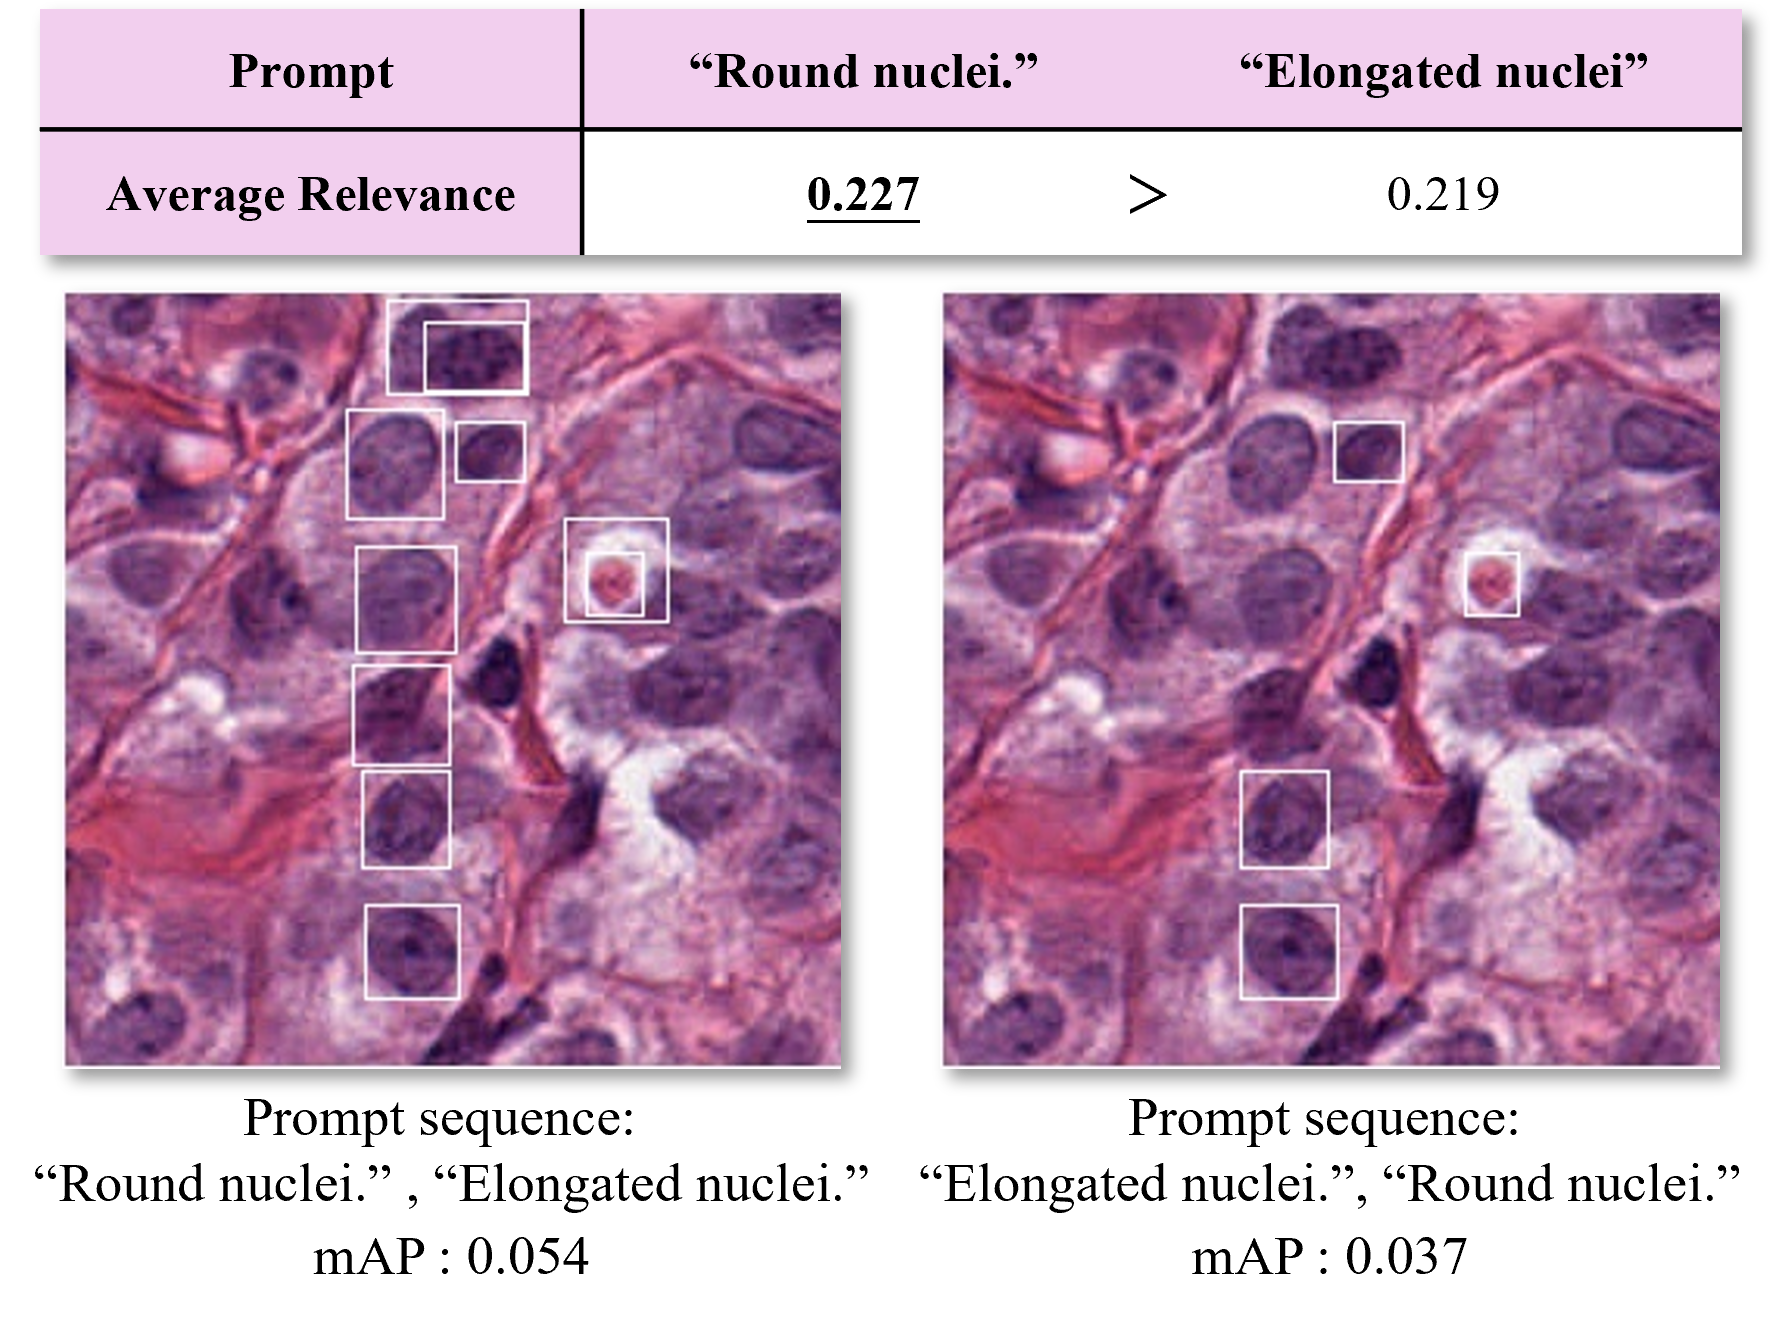
\includegraphics[width=0.95\linewidth]{chapters/PAPERS/nucleiprompter__TMI_final_version/xu2.png}
\caption{提示序列中较高相关性的提示放在前部可以提升 GLIP 的预测精度。mAP 在 MoNuSeg 测试集上统计。}
\label{fig:attrip_parelevance}
\end{figure}

这一现象说明提示序列并不是候选短语的简单集合。由于跨模态融合过程会受到序列上下文的影响，越符合当前图像域的提示越适合被放在前面。由此，本章将提示构造拆分为属性生成、属性增强和相关性排序三个步骤，以降低人工设计提示的主观性，并使提示序列能够随数据域变化而自动调整。

\section{AttriPrompter 自动属性提示框架}

AttriPrompter 的总体流程如图~\ref{fig:attrip_framework} 所示。首先，使用医学名词驱动 GLIP 产生粗略候选框，并利用这些候选框从无标注图像中裁剪细胞核区域；随后将裁剪区域输入 BLIP，通过视觉问答生成描述性词汇，再根据词频和属性类别筛选形状、颜色词。之后，使用语言模型对属性词进行同义增强和程度增强，将属性词与医学名词组合成候选提示；最后，依据候选提示和训练图像之间的平均图文相关性筛选并排序，得到输入 GLIP 的最终提示序列。

\begin{figure*}[t]
\centering
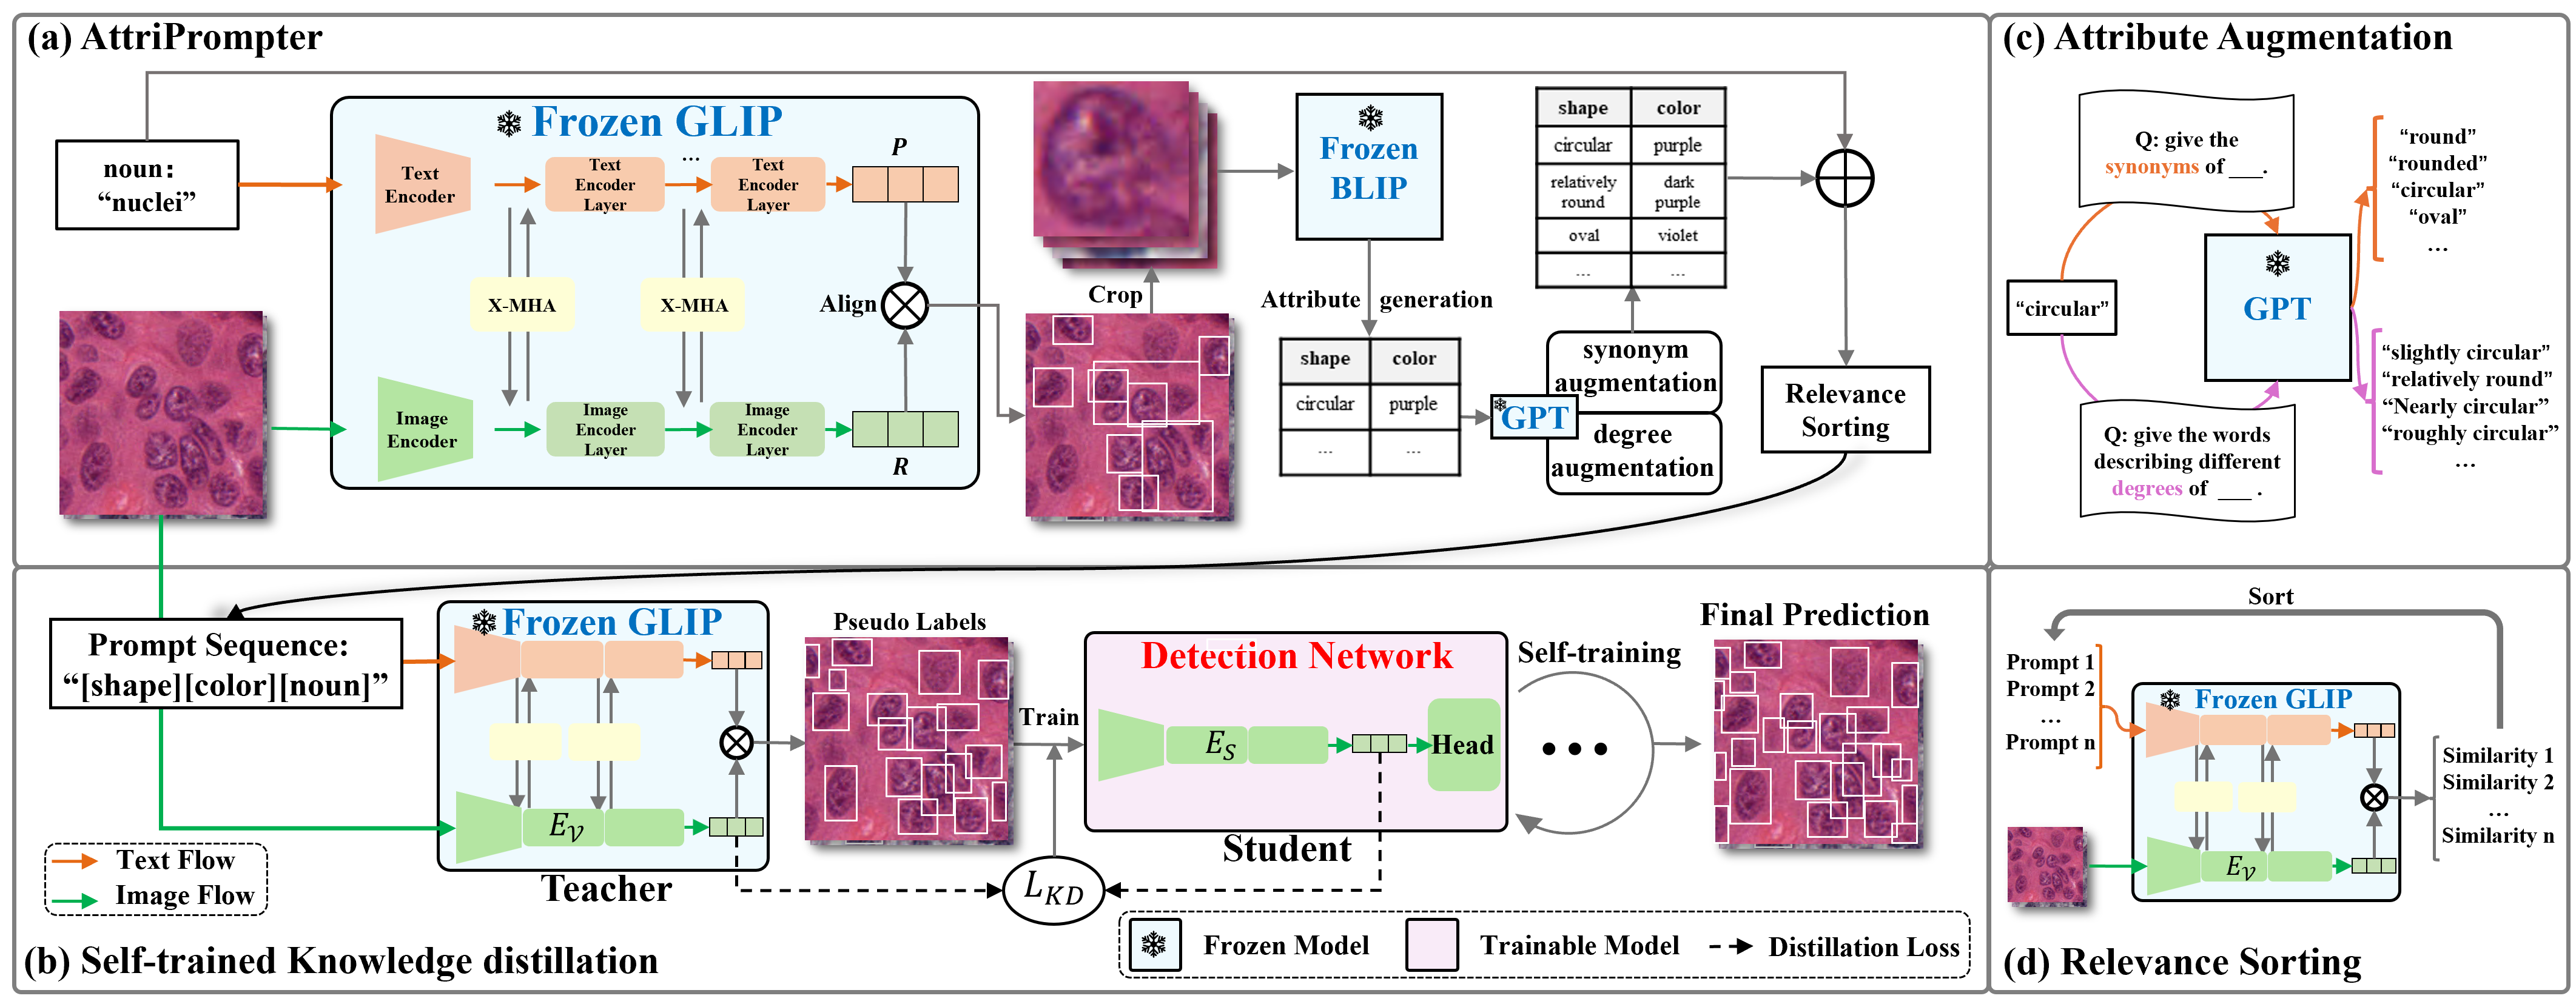
\includegraphics[width=\textwidth]{chapters/PAPERS/nucleiprompter__TMI_final_version/xu1.png}
\caption{AttriPrompter 与自训练知识蒸馏框架示意图。(a) 使用 GLIP 和 BLIP 自动生成属性，利用语言模型进行属性增强，并对候选提示进行相关性排序；(b) 基于自训练知识蒸馏进行迭代优化；(c) 属性增强过程；(d) 相关性排序过程。}
\label{fig:attrip_framework}
\end{figure*}

\subsection{属性生成}

属性生成的目标是从无标注图像中获得能够描述目标外观的词汇，避免依赖病理专家手工设计提示。具体步骤如下。

首先，将 ``nuclei'' 等医学名词作为初始提示输入 GLIP，得到细胞核的粗略候选框。此时的预测不要求具有很高的召回率，其作用是提供可供分析的候选区域。其次，将粗略候选框对应的图像区域裁剪为图像块，并输入冻结的 BLIP。BLIP 是一个兼具图像理解和文本生成能力的视觉语言模型，可以通过视觉问答回答图像块中目标的颜色和形状问题。最后，对 BLIP 生成的词汇进行词频统计和类别筛选，保留最能描述细胞核形状和颜色的属性词。

该流程具有两个优点。一方面，属性直接从目标域图像中提取，能够反映不同染色和成像条件下的细胞核外观；另一方面，属性生成依赖已经完成图文对齐的视觉语言模型，生成的词汇更有可能与 GLIP 的语义空间兼容。与完全人工设计相比，该方法减少了提示选择中的经验偏差，并保留了可解释性：每个最终提示都可以追溯到形状、颜色及其程度属性。

\subsection{属性增强}

属性生成得到的词汇数量和表达方式仍然有限。为扩大语义覆盖范围，AttriPrompter 对属性词执行同义增强和程度增强。

\textbf{同义增强。} 同义词可以在不改变基本语义的情况下提供多种语言表达。本章使用预训练语言模型对属性词进行扩展，例如将描述形状或颜色的常用词扩展为多个可能的自然语言表达。增强提示时使用的约束是：新词应当能够描述 H\&E 染色病理图像中的细胞核，而不是仅仅提供词典意义上的同义词。这样可以避免生成与目标外观无关的词汇。

\textbf{程度增强。} 仅使用 ``round'' 或 ``purple'' 等基本属性，仍然不能区分属性的强弱和程度。程度增强为每个属性添加更细粒度的描述，例如颜色的深浅、形状的圆整程度和弯曲程度。图~\ref{fig:attrip_augmentation} 中，同一框内的词表示基本语义相近的同义表达，不同框中的词表示属性程度不同。通过程度增强，候选集合覆盖了更宽的语义范围，提高了生成有效提示的概率。

\begin{figure}[t]
\centering
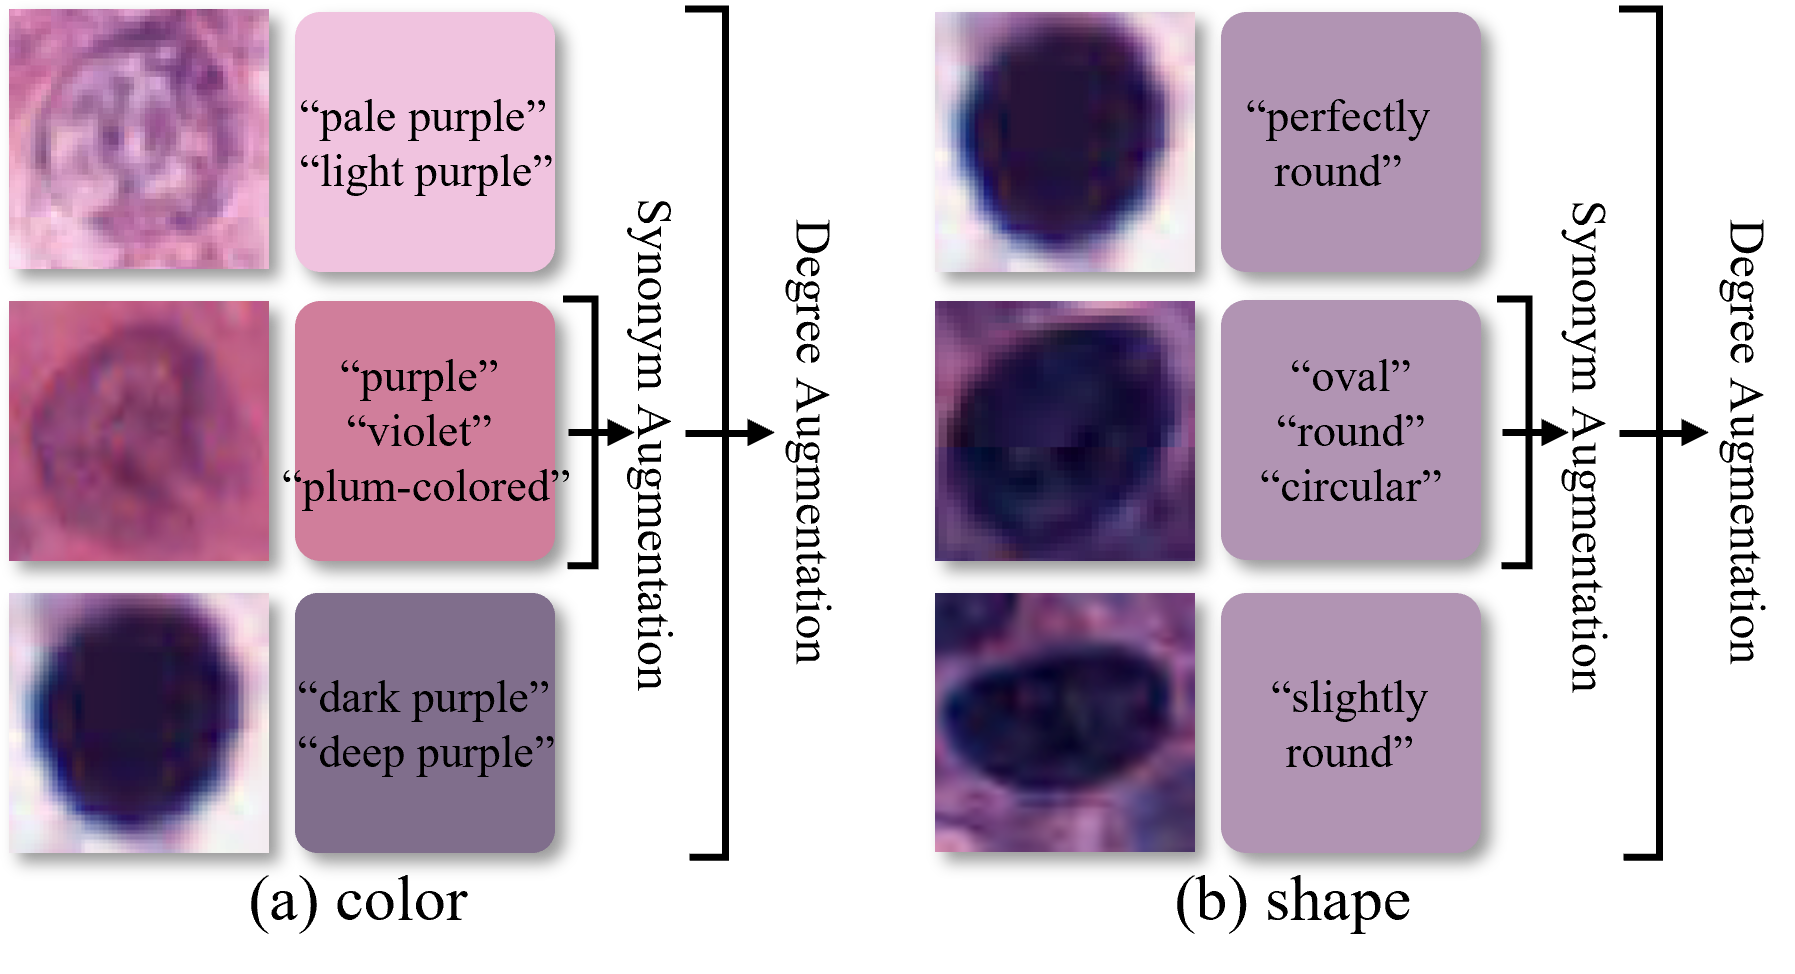
\includegraphics[width=0.95\linewidth]{chapters/PAPERS/nucleiprompter__TMI_final_version/xu3.png}
\caption{属性增强对不同细胞核外观的语义覆盖。(a) 对颜色 ``purple'' 的增强；(b) 对形状 ``round'' 的增强。同一框中的词表示同义表达，不同框中的词表示不同程度的属性描述。}
\label{fig:attrip_augmentation}
\vskip -0.15in
\end{figure}

\subsection{相关性排序}

将形状属性、颜色属性和医学名词按照模板 ``[shape] [color] [noun].'' 组合，可以形成候选检测提示。但是，程度增强也可能引入与当前图像域相关性较低的词汇。为降低无关提示带来的噪声，AttriPrompter 使用 GLIP 的视觉和文本编码结果计算提示相关性。

设训练图像 $x_i$ 中的候选区域集合为 $\mathcal{B}_i$，候选提示为 $t$。记区域 $b$ 的视觉嵌入为 $R_{i,b}=E_{\mathcal V}(x_i,b)$，提示的文本嵌入为 $P_t=E_{\mathcal T}(t)$，则候选提示在训练集上的平均相关性定义为：
\begin{equation}
\label{eq:attrip_relevance}
s(t)=\frac{1}{\sum_{i=1}^{n}|\mathcal{B}_i|}
\sum_{i=1}^{n}\sum_{b\in\mathcal{B}_i}
\frac{R_{i,b}\cdot P_t}{\|R_{i,b}\|_2\|P_t\|_2}.
\end{equation}

其中，$n$ 为用于提示生成和排序的训练图像数量。原论文为简化记号，将候选区域索引省略；式~\ref{eq:attrip_relevance} 将其显式写出，以说明相关性是对训练图像中的候选区域进行平均，而不是只计算整幅图像的单个相似度。根据 $s(t)$ 对候选提示进行降序排列，选取前 $N$ 个提示输入 GLIP。本章实验中 $N=9$，该值由 MoNuSeg 上的交叉验证确定。

相关性排序并不改变候选提示的文字内容，而是利用目标域图像确定提示的优先级。当相关性高的提示位于序列前部时，GLIP 的跨模态融合更容易先关注与当前图像外观一致的语义描述，从而改善初始预测的稳定性。

\section{自训练知识蒸馏}

\subsection{问题与总体思路}

H\&E 图像中的细胞核通常呈高密度排列，许多相邻实例之间只有很小的间隔。GLIP 虽然具有良好的目标级跨模态表示，但其预训练结构并不是专门为密集同类目标设计的，直接使用 GLIP 预测仍然容易出现漏检、误检和相邻实例重叠。若直接对目标域图像进行普通微调，又可能破坏 GLIP 原有的开放词汇知识。

为此，本章引入自训练知识蒸馏框架。GLIP 作为教师网络，通过 AttriPrompter 生成初始预测；这些预测被视为无人工标注的伪标签。随后，使用检测专用的学生网络学习伪标签，同时通过特征蒸馏损失约束学生特征与 GLIP 图像编码器特征之间的差异。学生网络的结构可以针对密集目标进行选择，实验中主要使用 YOLOX，也验证了 Mask R-CNN 的可替代性。学生网络收敛后重新生成伪标签，并开启下一轮训练，形成迭代自训练过程。

\subsection{教师网络、学生网络与训练目标}

设输入图像为 $x_i$，AttriPrompter 和 GLIP 产生的初始伪标签集合为
\begin{equation}
O_i=\{o_1,\ldots,o_{k_i}\},
\end{equation}
其中 $k_i$ 是第 $i$ 张图像中的伪标签数量。记 GLIP 的图像特征提取器为 $E_{\mathcal V}$，学生网络的特征提取器为 $E_{\mathcal S}$，学生检测头为 $\mathcal H$。知识蒸馏损失采用教师和学生特征之间的 $L_1$ 距离：
\begin{equation}
\label{eq:attrip_kd}
L_{KD}=\left\|E_{\mathcal V}(x_i)-E_{\mathcal S}(x_i)\right\|_1.
\end{equation}

学生网络的整体训练目标为：
\begin{equation}
\label{eq:attrip_student}
L_{\mathcal S}=\frac{1}{n}\sum_{i=1}^{n}
L_{Det}\left(O_i,\mathcal H(E_{\mathcal S}(x_i))\right)
+\alpha L_{KD},
\end{equation}
其中，$L_{Det}$ 表示学生检测网络的检测损失，$\alpha$ 为知识蒸馏损失权重。本章实验将 YOLOX 的特征提取器修改为与 GLIP 图像编码器相同的结构，并使用 GLIP 预训练权重进行初始化，以便进行特征对齐。需要强调的是，GLIP 在这里是教师网络，YOLOX 或 Mask R-CNN 是学生检测网络；SKD 的作用不是重新训练 GLIP，而是将其目标级知识迁移到更适合密集目标检测的网络中。

\subsection{迭代自训练}

第一轮训练结束后，使用已经收敛的学生网络重新预测训练图像，得到更新后的伪标签集合 $O_i^{(r+1)}$。随后以更新后的伪标签启动下一轮学生网络训练：
\begin{equation}
\label{eq:attrip_iterative}
L_{\mathcal S^{(r+1)}}=\frac{1}{n}\sum_{i=1}^{n}
L_{Det}\left(O_i^{(r+1)},
\mathcal H^{(r+1)}(E_{\mathcal S^{(r+1)}}(x_i))\right)
+\alpha L_{KD}.
\end{equation}

从优化角度看，这一过程可以理解为交替更新伪标签和学生网络参数：固定当前模型生成伪标签，再固定伪标签训练下一轮模型。由于后续轮次使用了学生网络对目标形态的建模能力，预测框的位置和数量可以逐步得到修正。实际实验中并非轮次越多越好，因此本章同时报告不同自训练轮次的结果，并根据验证集表现选择最终轮次。

\section{实验设置}

\subsection{数据集与数据划分}

\textbf{MoNuSeg。} MoNuSeg 包含 30 张 $1000\times1000$ 像素的细胞核图像，每张图像平均包含约 658 个细胞核。按照数据集原始划分，使用 16 张图像训练，14 张图像测试；训练过程中每个 epoch 随机选择 4 张图像用于验证。每张大图提取 16 个具有重叠区域的 $256\times256$ 图像块，并随机裁剪为 $224\times224$ 作为模型输入。训练图像仅用于自动提示生成和伪标签自训练，测试图像及其真实标注只用于最终评估。

\textbf{CoNSeP。} CoNSeP 是面向结直肠细胞核分割和表型分析的数据集，包含 41 张 $1000\times1000$ 像素的 H\&E 染色图像，这些图像来自 16 张结直肠腺癌全视野切片。除非另有说明，本章沿用与 MoNuSeg 相同的预处理方式。按照数据集默认划分，使用 26 张图像训练、1 张图像验证、14 张图像测试。

\subsection{评价指标}

本章遵循 COCO 评价协议，采用平均精度 mAP、IoU 阈值为 0.50 的 AP50、IoU 阈值为 0.75 的 AP75，以及平均召回率 AR 作为主要检测指标。mAP 综合多个 IoU 阈值下的精度，反映预测框定位精度与置信度排序的整体质量；AP50 更关注较宽松的目标匹配，AP75 对定位误差更敏感；AR 则用于衡量模型发现目标的能力。对于伪标签分析，额外使用每个伪标签与真实实例中最大 IoU 的平均值 $\mathrm{mIoU}_{\mathrm{nearest}}$，以区分“定位较准但数量不足”和“定位本身不准”两类情况。

\subsection{实现细节}

除非另有说明，实验使用 4 张具有 24 GB 显存的 NVIDIA RTX 3090 GPU。AttriPrompter 的属性生成使用在 ViT-B 和 CapFilt-L 上微调的 BLIP VQA 权重，视觉问答问题分别为 ``what is the color of the nuclei'' 和 ``what is the shape of the nuclei''。属性增强使用 ChatGPT 3.5，提示内容分别要求生成“能够描述 H\&E 染色病理图像中细胞核的同义词”和“描述某一属性不同程度的词语”。相关性排序选取 $N=9$ 个提示。主干视觉语言模型使用 GLIP-L。

在 SKD 中，将 YOLOX 的特征提取器替换为与 GLIP 图像编码器一致的结构，并使用 GLIP 预训练参数初始化；学生网络的其他训练设置采用 YOLOX 默认配置。知识蒸馏权重 $\alpha=1$，该值通过 MoNuSeg 上的四折交叉验证确定。若未特别说明，每张图像最多保留 20 个伪标签。不同的自训练轮次均使用相同的评价协议，避免把轮次变化和评价方法变化混在一起。

\section{实验结果与分析}

\subsection{与现有方法的比较}

表~\ref{tab:attrip_comparison} 汇总了本章方法与全监督、弱监督以及无监督方法的比较结果。带有 ``*'' 的方法基于医学图像，带有 ``**'' 的方法专门针对 H\&E 图像，其余方法原本面向自然图像，经过适配后用于细胞核检测。弱监督方法使用点标注作为监督信号；本章按照细胞核实例掩膜的中心生成点标注，以保持点监督定义的一致性。

\begin{table}[t]
\caption{MoNuSeg 与 CoNSeP 数据集上的检测结果（mAP、AP50、AP75 和 AR）。带 ``*'' 的方法基于医学图像，带 ``**'' 的方法专门针对 H\&E 图像。无监督方法中的最优结果以粗体表示。}
\label{tab:attrip_comparison}
\begin{center}
\resizebox{\columnwidth}{!}{
\begin{tabular}{ccccccccc}
\toprule[1.5pt]
\multirow{2}{*}{\textbf{方法}} & \multicolumn{4}{c}{\textbf{MoNuSeg}} & \multicolumn{4}{c}{\textbf{CoNSeP}} \\ \cmidrule(r){2-5} \cmidrule(r){6-9}
 & \textbf{mAP} & \textbf{AP50} & \textbf{AP75} & \textbf{AR} & \textbf{mAP} & \textbf{AP50} & \textbf{AP75} & \textbf{AR} \\ \midrule[1.2pt]
\multicolumn{9}{c}{\textbf{全监督基线}} \\
\textbf{YOLOX} & 0.447 & 0.832 & 0.437 & 0.528 & 0.388 & 0.726 & 0.384 & 0.495 \\ \hline
\multicolumn{9}{c}{\textbf{弱监督方法}} \\
\textbf{WSPointA(2019)**\cite{qu2019weakly}} & 0.341 & 0.683 & 0.272 & 0.423 & 0.301 & 0.593 & 0.277 & 0.362 \\
\textbf{WSPPointA(2020)**\cite{qu2020weakly}} & 0.367 & 0.763 & 0.302 & 0.453 & 0.308 & 0.607 & 0.281 & 0.373 \\
\textbf{WSMixedA(2020)**\cite{qu2020nuclei}} & 0.374 & 0.771 & 0.374 & 0.488 & 0.330 & 0.653 & 0.307 & 0.412 \\
\textbf{WNSeg(2022)**\cite{liu2022weakly}} & 0.404 & 0.797 & 0.416 & 0.505 & 0.364 & 0.675 & 0.329 & 0.434 \\ \hline
\multicolumn{9}{c}{\textbf{无监督方法：非视觉语言预训练模型}} \\
\textbf{SSNS(2020)**\cite{sahasrabudhe2020self}} & 0.354 & 0.739 & 0.288 & 0.441 & 0.243 & 0.458 & 0.215 & 0.294 \\
\textbf{PDAM(2020)*\cite{liu2020pdam}} & 0.275 & 0.588 & 0.228 & 0.380 & 0.166 & 0.364 & 0.132 & 0.298 \\
\textbf{DARCNN(2021)*\cite{hsu2021darcnn}} & 0.262 & 0.476 & 0.267 & 0.356 & 0.173 & 0.388 & 0.129 & 0.310 \\
\textbf{Freesolo(2022)\cite{wang2022freesolo}} & 0.292 & 0.607 & 0.248 & 0.393 & 0.222 & 0.393 & 0.246 & 0.370 \\
\textbf{SOP(2022)*\cite{le2022unsupervised}} & 0.235 & 0.609 & 0.096 & 0.351 & 0.171 & 0.387 & 0.127 & 0.304 \\
\textbf{PSM(2022)**\cite{chen2022unsupervised}} & 0.227 & 0.447 & 0.218 & 0.375 & 0.142 & 0.323 & 0.102 & 0.286 \\
\textbf{CutLER(2023)\cite{wang2023cut}} & 0.115 & 0.213 & 0.117 & 0.184 & 0.089 & 0.181 & 0.049 & 0.155 \\ \hline
\multicolumn{9}{c}{\textbf{无监督方法：视觉语言预训练模型}} \\
\textbf{VL-PLM(2022)\cite{zhao2022exploiting}} & 0.333 & 0.582 & 0.342 & 0.501 & 0.159 & 0.357 & 0.120 & 0.291 \\
\textbf{VLDet(2023)\cite{lin2022learning}} & 0.173 & 0.407 & 0.112 & 0.263 & 0.110 & 0.296 & 0.053 & 0.245 \\
\textbf{MIU-VL(2023)*\cite{qin2022medical}} & 0.070 & 0.118 & 0.076 & 0.126 & 0.066 & 0.133 & 0.045 & 0.121 \\
\textbf{VLPM-NuD(2023)**\cite{wu2023zeroshot}} & 0.416 & 0.808 & 0.382 & 0.502 & 0.359 & 0.668 & 0.363 & 0.480 \\
\textbf{本章方法**} & \textbf{0.425} & \textbf{0.819} & \textbf{0.401} & \textbf{0.511} & \textbf{0.367} & \textbf{0.669} & \textbf{0.376} & \textbf{0.488} \\ \bottomrule[1.5pt]
\end{tabular}
}
\end{center}
\end{table}

本章方法在两个数据集上均取得了无监督方法中的最佳综合结果，并接近全监督 YOLOX。非视觉语言方法通常需要依赖尺寸、阈值或域适配假设，在密集同类目标上难以同时保持精度和召回率。VL-PLM 和 VLDet 具有开放词汇能力，但没有针对 H\&E 图像进行提示和密集目标适配，因此表现有限。MIU-VL 同样基于 GLIP，但其自动提示更偏向于位置属性，适合稀疏目标检测，在细胞核密集分布场景中可能引入额外干扰。

AttriPrompter 的优势来自三个方面：自动属性生成使提示能够描述目标域外观；同义和程度增强扩大了细粒度语义覆盖；相关性排序降低了低相关提示对 GLIP 跨模态融合的干扰。进一步结合 SKD 后，学生检测器可以利用 GLIP 的目标级先验，并通过多轮伪标签更新适应密集细胞核结构。图~\ref{fig:attrip_comparison} 给出了不同方法的检测可视化结果。

\begin{figure*}[t]
\centering
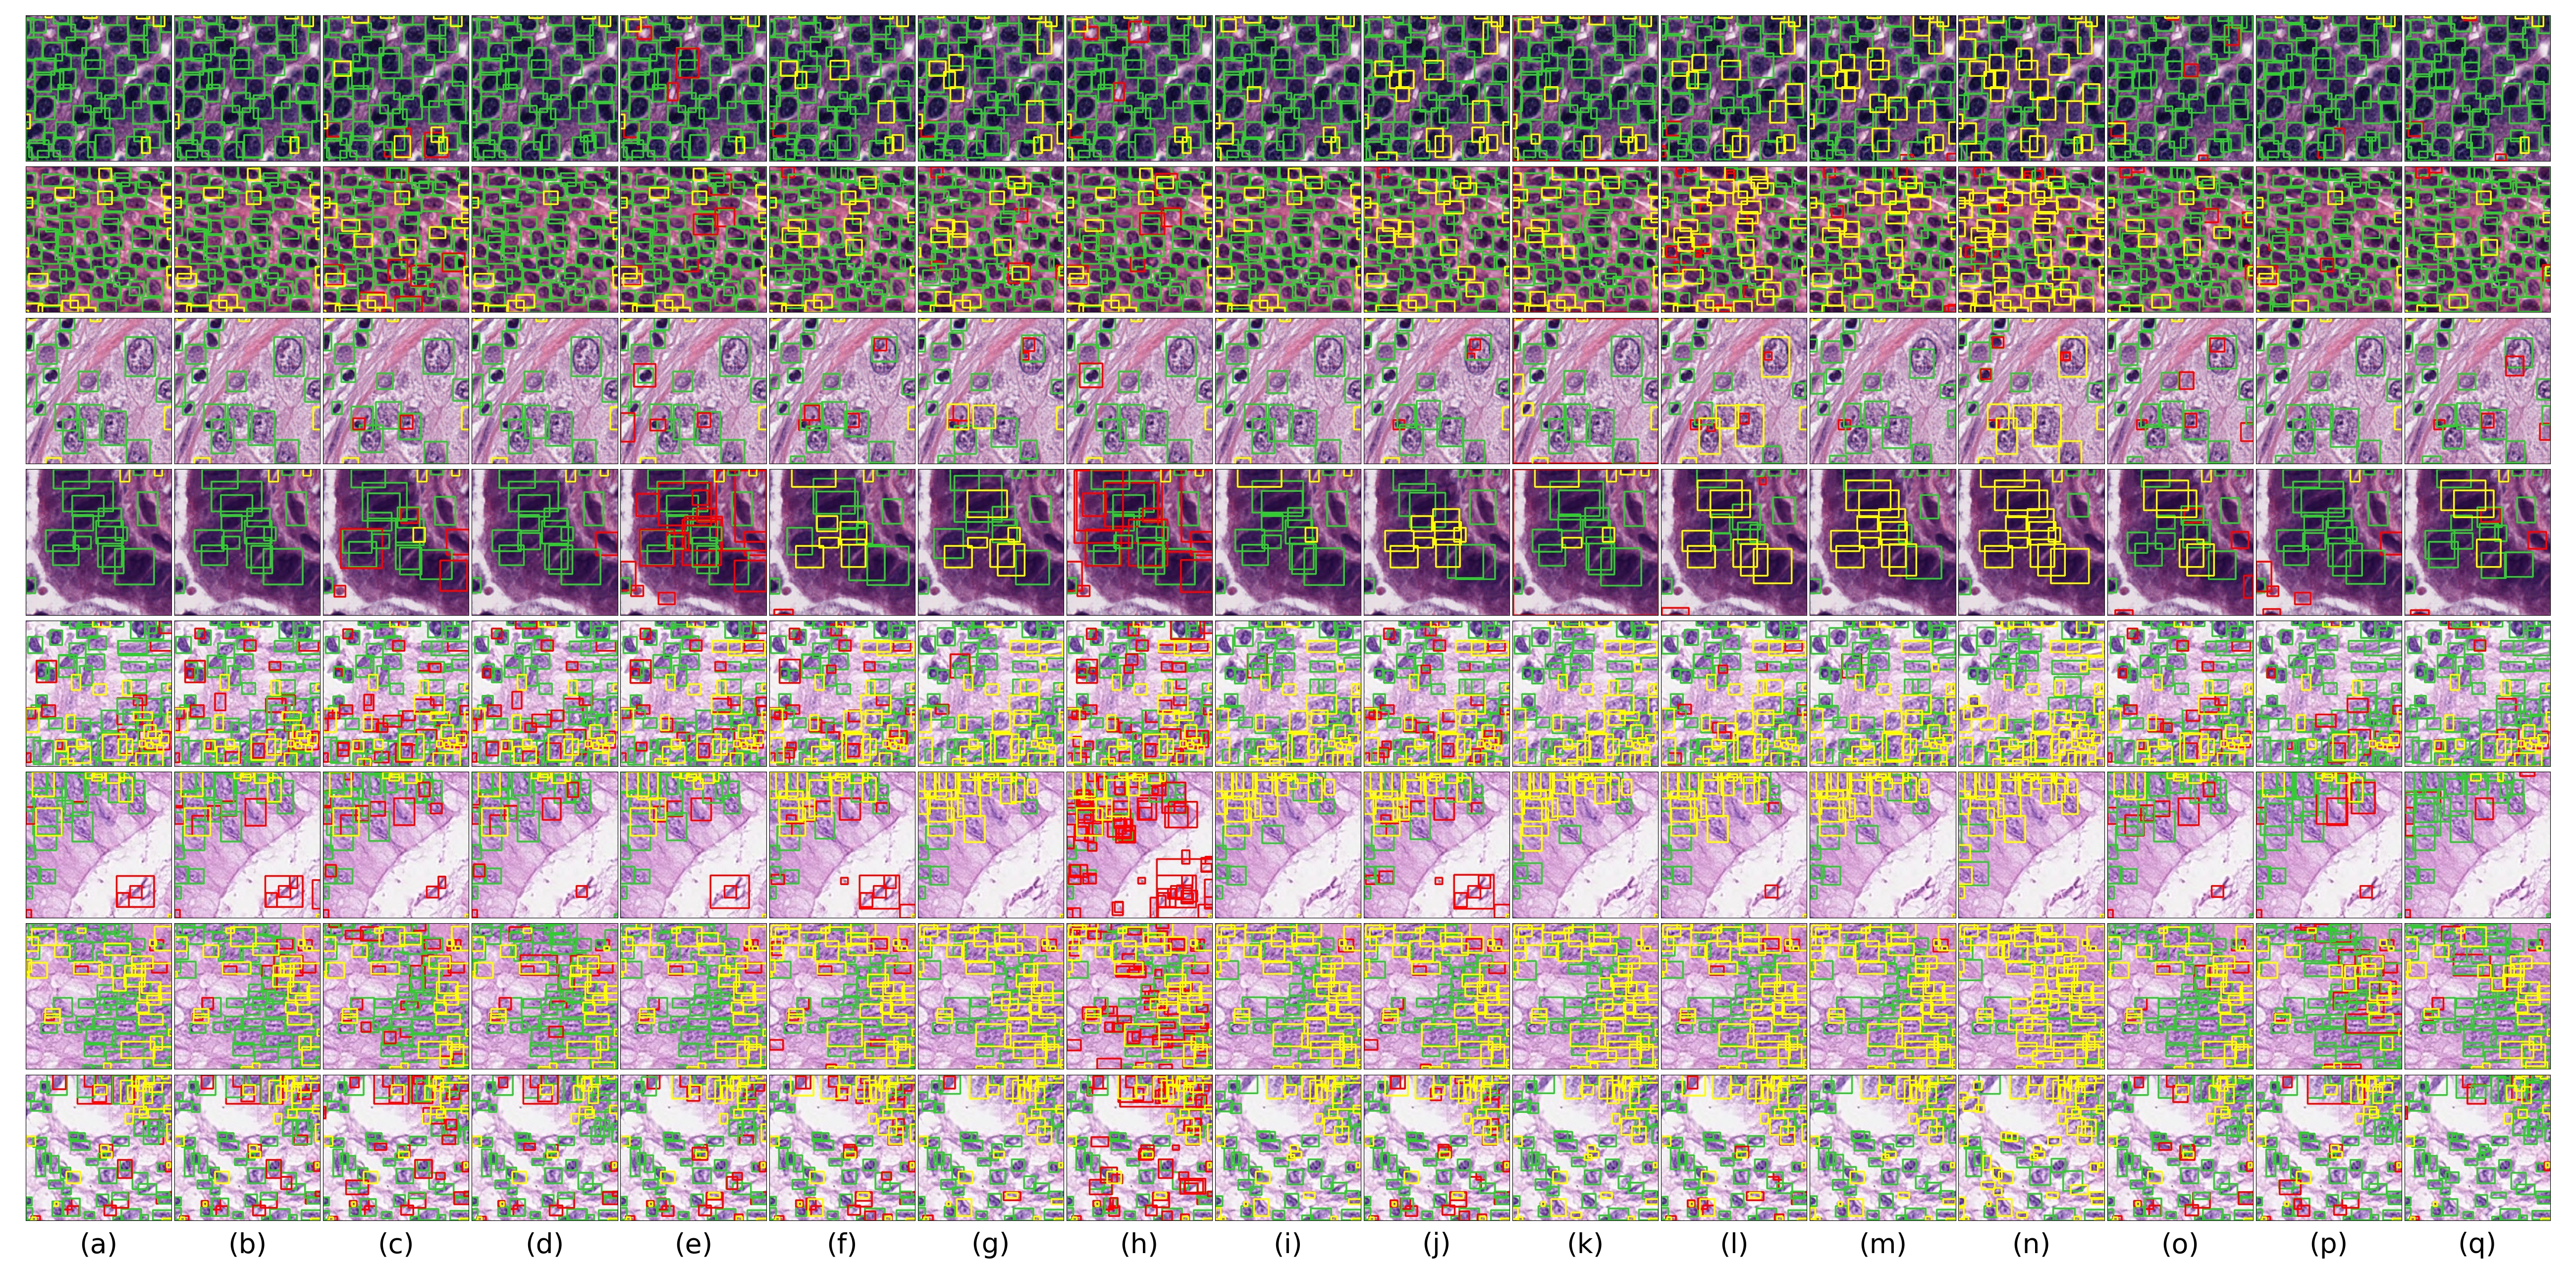
\includegraphics[width=\linewidth]{chapters/PAPERS/nucleiprompter__TMI_final_version/xu4.png}
\caption{不同方法的检测可视化结果。前四行为 MoNuSeg，后四行为 CoNSeP。绿色、红色和黄色框分别表示真阳性、假阳性和假阴性。}
\label{fig:attrip_comparison}
\end{figure*}

\subsection{自动提示与人工提示}

为直接评估提示质量，本节不引入 SKD，而是将不同提示序列直接输入 GLIP，并在相同设置下进行零样本检测。人工提示由三位病理专家分别设计，结果取平均值；其描述通常包含染色质形态、核仁以及深蓝或紫色等颜色信息。自动提示则分别使用医学名词、形状属性、颜色属性以及形状和颜色的组合。表~\ref{tab:attrip_prompt} 中的 ``Aug.'' 表示经过语言模型增强。

\begin{table}[t]
\caption{自动提示与人工提示的比较。该实验不使用 SKD，用于直接评估提示设计质量。最优结果以粗体表示。}
\label{tab:attrip_prompt}
\begin{center}
\resizebox{0.9\columnwidth}{!}{
\renewcommand{\arraystretch}{1.1}
\begin{tabular}{ccccccc}
\toprule[1.5pt]
\multicolumn{3}{c}{\multirow{2}{*}{\textbf{提示设计}}} & \multicolumn{4}{c}{\textbf{MoNuSeg}} \\ \cline{4-7}
\multicolumn{3}{c}{} & \textbf{mAP} & \textbf{AP50} & \textbf{AP75} & \textbf{AR} \\ \midrule[1.2pt]
\multicolumn{3}{c}{\textbf{人工设计}} & 0.151 & 0.259 & 0.166 & 0.210 \\ \hline
\multirow{10}{*}{\textbf{自动生成}} & \multicolumn{2}{c}{\textbf{MIU-VL(2023)\cite{qin2022medical}}} & 0.070 & 0.118 & 0.076 & 0.126 \\ \cline{2-7}
 & \textbf{属性} & \textbf{名词} & & & & \\ \cline{2-7}
 & \multirow{2}{*}{\textbf{无}} & \textbf{``Nuclei.''} & 0.034 & 0.057 & 0.038 & 0.058 \\
 & & \textbf{Aug. [noun.]} & 0.029 & 0.054 & 0.029 & 0.059 \\ \cline{2-7}
 & \textbf{[shape]} & \textbf{``Nuclei.''} & 0.097 & 0.181 & 0.097 & 0.155 \\
 & \textbf{Aug. [shape]} & \textbf{``Nuclei.''} & 0.124 & 0.255 & 0.124 & 0.191 \\ \cline{2-7}
 & \textbf{[color]} & \textbf{``Nuclei.''} & 0.009 & 0.016 & 0.010 & 0.024 \\
 & \textbf{Aug. [color]} & \textbf{``Nuclei.''} & 0.064 & 0.115 & 0.066 & 0.112 \\ \cline{2-7}
 & \textbf{[shape][color]} & \textbf{``Nuclei.''} & 0.155 & 0.285 & 0.152 & \textbf{0.239} \\
 & \textbf{Aug. [shape][color]} & \textbf{``Nuclei.''} & \textbf{0.179} & \textbf{0.310} & \textbf{0.193} & 0.220 \\ \bottomrule[1.5pt]
\end{tabular}
}
\end{center}
\end{table}

结果显示，人工提示能够取得一定性能，但依赖设计者经验，难以保证不同数据域之间的一致性。只使用类别名时性能最低；加入形状或颜色属性后性能总体提升；同时使用形状和颜色时效果最好。值得注意的是，名词同义扩展并未带来收益，可能原因是 ``cyteblast'' 和 ``karyon'' 等生僻词没有充分出现在 GLIP 的预训练语料中。相比之下，常见自然语言属性词更容易与预训练视觉语义形成对应关系。MIU-VL 的表现较低，也说明适合稀疏医学目标的位置类属性不一定适合密集细胞核检测。

\subsection{AttriPrompter 组件消融}

表~\ref{tab:attrip_promptcom} 分别去除同义增强、程度增强和相关性排序，分析三个组件的独立作用及组合效果。所有设置均不使用 SKD，以排除学生网络和自训练过程的影响。

\begin{table}[t]
\caption{AttriPrompter 组件消融实验。该实验不使用 SKD。最优结果以粗体表示。}
\label{tab:attrip_promptcom}
\begin{center}
\resizebox{0.9\columnwidth}{!}{
\begin{tabular}{ccccccc}
\toprule[1.5pt]
\textbf{同义增强} & \textbf{程度增强} & \textbf{相关性排序} & \textbf{mAP} & \textbf{AP50} & \textbf{AP75} & \textbf{AR} \\ \midrule[1.2pt]
 & & & 0.150 & 0.275 & 0.150 & 0.228 \\
\checkmark & & & 0.160 & 0.285 & 0.173 & 0.201 \\
 & \checkmark & & 0.176 & 0.304 & 0.187 & 0.213 \\
 & & \checkmark & 0.155 & 0.290 & 0.152 & \textbf{0.239} \\
\checkmark & & \checkmark & 0.174 & 0.301 & 0.188 & 0.210 \\
 & \checkmark & \checkmark & 0.178 & \textbf{0.314} & 0.187 & 0.217 \\
\checkmark & \checkmark & & 0.177 & 0.309 & \textbf{0.193} & 0.220 \\
\checkmark & \checkmark & \checkmark & \textbf{0.179} & 0.310 & \textbf{0.193} & 0.220 \\ \bottomrule[1.5pt]
\end{tabular}
}
\end{center}
\vskip -0.15in
\end{table}

三个组件组合使用时 mAP 达到 0.179，是表中最高值。程度增强和相关性排序的组合在 AP50 上达到最高值，说明细粒度属性和提示顺序分别改善了候选语义和序列上下文。仅使用同义增强的设置与第三章中较早的自动提示方案相近，性能提升相对有限。总体而言，程度增强是本章相对于基础自动属性提示的重要扩展，而相关性排序则进一步利用了 GLIP 对提示顺序的敏感性。

\subsection{不同伪标签生成方式的自训练}

为了区分“伪标签质量”和“学生网络自训练能力”的作用，本节比较 Superpixels、MIU-VL 和 AttriPrompter 三种伪标签来源。除伪标签生成方法外，三个设置均使用相同的 YOLOX 自训练框架。表~\ref{tab:attrip_selftraining} 中，Round 0 表示直接将初始伪标签与真实标注比较；Round 1 表示学生网络完成第一轮收敛后的结果；后续轮次使用前一轮学生网络生成新的伪标签。AttriPrompter 列的结果不使用知识蒸馏，以便单独考察伪标签和自训练过程。

\begin{table}[t]
\caption{采用不同伪标签生成方式进行自训练的结果。AttriPrompter（Ours）列不使用知识蒸馏。最优结果以粗体表示。}
\label{tab:attrip_selftraining}
\begin{center}
\resizebox{\columnwidth}{!}{
\begin{tabular}{ccccccccccccc}
\toprule[1.5pt]
\multirow{2}{*}{\textbf{轮次}} & \multicolumn{4}{c}{\textbf{Superpixels}} & \multicolumn{4}{c}{\textbf{MIU-VL}} & \multicolumn{4}{c}{\textbf{AttriPrompter}} \\ \cmidrule(r){2-5} \cmidrule(r){6-9} \cmidrule(r){10-13}
 & \textbf{mAP} & \textbf{AP50} & \textbf{AP75} & \textbf{AR} & \textbf{mAP} & \textbf{AP50} & \textbf{AP75} & \textbf{AR} & \textbf{mAP} & \textbf{AP50} & \textbf{AP75} & \textbf{AR} \\ \midrule[1.2pt]
\textbf{Round 0} & 0.027 & 0.075 & 0.012 & 0.035 & 0.070 & 0.118 & 0.076 & 0.126 & 0.179 & 0.310 & 0.193 & 0.220 \\
\textbf{Round 1} & 0.260 & 0.612 & 0.162 & 0.373 & 0.221 & 0.486 & 0.208 & 0.370 & 0.302 & 0.693 & 0.248 & 0.393 \\
\textbf{Round 2} & 0.272 & 0.617 & 0.183 & 0.392 & 0.242 & 0.495 & 0.239 & 0.381 & 0.358 & 0.724 & 0.326 & 0.430 \\
\textbf{Round 3} & 0.284 & 0.655 & 0.169 & 0.404 & 0.266 & 0.511 & 0.265 & 0.409 & \textbf{0.363} & 0.730 & 0.327 & 0.433 \\
\textbf{Round 4} & 0.279 & 0.614 & 0.213 & 0.389 & 0.269 & 0.515 & 0.266 & 0.416 & 0.361 & \textbf{0.732} & \textbf{0.331} & \textbf{0.435} \\ \bottomrule[1.5pt]
\end{tabular}
}
\end{center}
\vskip -0.15in
\end{table}

Superpixels 和 MIU-VL 产生的初始伪标签质量较低，虽然经过自训练后性能明显提升，但仍低于 AttriPrompter。AttriPrompter 在 Round 0 已具有较好的初始结果，经过多轮训练后 mAP 在 Round 3 达到 0.363，之后略有回落。因此，自训练过程能够改善初始伪标签，但最终性能的上限主要由初始伪标签是否具有可靠的目标语义决定。这一结果也说明本章的核心贡献并不是单纯选择更强的学生网络，而是通过属性提示充分利用 GLIP 的先验知识。

\subsection{伪标签与真实标签的质量比较}

表~\ref{tab:attrip_pseudoreal} 直接比较初始伪标签与测试集真实标注。由于密集细胞核会造成较多漏检，初始伪标签的 AR 和 AP 不高；但是，$\mathrm{mIoU}_{\mathrm{nearest}}$ 相对较高，说明已经被检测到的伪标签通常具有较好的定位精度。因此，初始伪标签的主要问题是召回率不足，而不是所有预测框都严重偏离真实细胞核。

\begin{table}[t]
\caption{初始伪标签与真实标注的直接比较。}
\label{tab:attrip_pseudoreal}
\begin{center}
\resizebox{0.86\columnwidth}{!}{
\begin{tabular}{cccccc}
\toprule[1.5pt]
\textbf{数据集} & \textbf{mAP} & \textbf{AP50} & \textbf{AP75} & \textbf{AR} & $\textbf{mIoU}_{\textbf{nearest}}$ \\ \midrule[1.2pt]
\textbf{MoNuSeg} & 0.178 & 0.312 & 0.195 & 0.217 & 0.742 \\
\textbf{CoNSeP} & 0.096 & 0.178 & 0.101 & 0.146 & 0.690 \\ \bottomrule[1.5pt]
\end{tabular}
}
\end{center}
\vskip -0.1in
\end{table}

进一步地，表~\ref{tab:attrip_semisupervised} 比较了在 SKD 框架中使用不同数量真实实例标注的结果。表中的百分比按每张训练图像的实例数量计算，例如 50\% 表示每张训练图像中一半细胞核实例使用真实框标注。AttriPrompter 伪标签的 mAP 为 0.425，高于使用 10\% 真实实例标注的结果，说明自动伪标签能够减少大量人工标注；但其整体性能仍未超过使用 50\% 真实标注的设置，表明伪标签的召回率仍有提升空间。

\begin{table}[t]
\caption{AttriPrompter 伪标签与不同比例真实标签在 SKD 框架中的比较。最优和次优结果分别以粗体和下划线表示。}
\label{tab:attrip_semisupervised}
\begin{center}
\resizebox{0.78\columnwidth}{!}{
\begin{tabular}{cccccc}
\toprule[1.5pt]
\multicolumn{2}{c}{\textbf{标签类型}} & \textbf{mAP} & \textbf{AP50} & \textbf{AP75} & \textbf{AR} \\ \midrule[1.2pt]
\multirow{4}{*}{\textbf{真实标签}} & \textbf{1\%} & 0.185 & 0.588 & 0.037 & 0.276 \\
 & \textbf{5\%} & 0.345 & 0.728 & 0.279 & 0.429 \\
 & \textbf{10\%} & 0.378 & 0.761 & 0.332 & 0.458 \\
 & \textbf{50\%} & \textbf{0.443} & \textbf{0.819} & \textbf{0.448} & \textbf{0.516} \\ \midrule
\multicolumn{2}{c}{\textbf{伪标签}} & {\ul 0.425} & \textbf{0.819} & {\ul 0.401} & {\ul 0.511} \\ \bottomrule[1.5pt]
\end{tabular}
}
\end{center}
\vskip -0.15in
\end{table}

\subsection{最优提示词分析}

相关性排序的一个优点是可以输出每个提示的相关性分数和单提示预测结果。表~\ref{tab:attrip_detailprompt} 展示 MoNuSeg 上相关性最高的 15 个候选提示，其中前 9 个提示在交叉验证后被选为最终提示，后续提示仅作为对照。结果显示，包含 ``slightly round''、``dark purple''、``moderately round'' 和 ``circular'' 的提示相对有效；这些词既符合 H\&E 染色细胞核的常见外观，也较容易与 GLIP 预训练阶段的自然语言形成对应。相反，``elliptical'' 和 ``elongated'' 等词在自然语言语料中的使用频率较低，可能导致跨模态匹配较弱。

\begin{table}[t]
\caption{MoNuSeg 上最优提示词的定量分析。前 9 个提示通过交叉验证选取，后续提示被舍弃并以灰色标记。}
\label{tab:attrip_detailprompt}
\begin{center}
\resizebox{0.98\columnwidth}{!}{
\begin{tabular}{cccc}
\toprule[1.5pt]
\textbf{排序} & \textbf{提示词} & \textbf{相关性} & \textbf{单提示 mAP} \\ \midrule[1.2pt]
1 & ``slightly round dark purple nuclei.'' & 0.317 & 0.116 \\
2 & ``slightly round purple nuclei.'' & 0.315 & 0.128 \\
3 & ``moderately round purple nuclei.'' & 0.312 & 0.104 \\
4 & ``moderately round dark purple nuclei.'' & 0.311 & 0.103 \\
5 & ``slightly round violet nuclei.'' & 0.311 & 0.099 \\
6 & ``circular purple nuclei.'' & 0.306 & 0.063 \\
7 & ``circular dark purple nuclei.'' & 0.304 & 0.067 \\
8 & ``circular violet nuclei.'' & 0.303 & 0.061 \\
9 & ``moderately round violet nuclei.'' & 0.302 & 0.057 \\
\rowcolor{lightgray} 10 & ``mostly round rich purple nuclei.'' & 0.299 & 0.054 \\
\rowcolor{lightgray} 11 & ``moderately round rich purple nuclei.'' & 0.299 & 0.051 \\
\rowcolor{lightgray} 12 & ``elliptical purple-blue nuclei.'' & 0.298 & 0.041 \\
\rowcolor{lightgray} 13 & ``elongated dark purple nuclei.'' & 0.296 & 0.040 \\
\rowcolor{lightgray} 14 & ``slightly circular plum-colored nuclei.'' & 0.294 & 0.033 \\
\rowcolor{lightgray} 15 & ``elliptical vibrant purple nuclei.'' & 0.294 & 0.032 \\
\rowcolor{lightgray} \multicolumn{4}{c}{\cellcolor{lightgray}...} \\ \bottomrule[1.5pt]
\end{tabular}
}
\end{center}
\vskip -0.15in
\end{table}

\subsection{知识蒸馏损失消融}

为了验证 $L_{KD}$ 是否能够帮助学生网络保留 GLIP 的目标级先验，表~\ref{tab:attrip_kd} 在人工提示、仅使用 ``Nuclei.'' 和完整 AttriPrompter 三种提示设置下分别去除或加入知识蒸馏损失。无论使用何种提示，加入 $L_{KD}$ 后 mAP 和 AR 均得到提升；在完整 AttriPrompter 下，mAP 从 0.412 提升到 0.425，说明知识蒸馏可以有效改善自训练结果。

\begin{table}[t]
\caption{知识蒸馏损失 $L_{KD}$ 的消融实验。不使用 $L_{KD}$ 时，学生网络仅由检测损失 $L_{Det}$ 训练。最优结果以粗体表示。}
\label{tab:attrip_kd}
\begin{center}
\resizebox{0.9\columnwidth}{!}{
\begin{tabular}{cccccc}
\toprule[1.5pt]
\textbf{提示设计} & $\boldsymbol{L_{KD}}$ & \textbf{mAP} & \textbf{AP50} & \textbf{AP75} & \textbf{AR} \\ \midrule[1.2pt]
\multirow{2}{*}{\textbf{人工提示}} & & 0.409 & 0.801 & 0.383 & 0.493 \\
 & \checkmark & 0.418 & 0.811 & 0.392 & 0.504 \\ \hline
\multirow{2}{*}{\textbf{``Nuclei.''}} & & 0.324 & 0.696 & 0.316 & 0.381 \\
 & \checkmark & 0.352 & 0.711 & 0.334 & 0.414 \\ \hline
\multirow{2}{*}{\textbf{AttriPrompter}} & & 0.412 & 0.805 & 0.385 & 0.498 \\
 & \checkmark & \textbf{0.425} & \textbf{0.819} & \textbf{0.401} & \textbf{0.511} \\ \bottomrule[1.5pt]
\end{tabular}
}
\end{center}
\end{table}

\subsection{不同学生检测网络结构}

SKD 的学生网络并不限定为 YOLOX。为验证方法的结构可迁移性，本节将学生网络替换为 Mask R-CNN，并保持伪标签生成、蒸馏损失和自训练流程不变。Mask R-CNN 训练时每张图像最多使用 100 个真实或伪标签实例，RPN 在训练和测试阶段的非极大值抑制阈值分别设置为 0.9 和 0.7，其余参数采用 COCO 默认配置。表~\ref{tab:attrip_architecture} 显示，使用 Mask R-CNN 时本章方法仍然优于相同学生结构下的 VLPM-NuD，说明性能提升主要来自提示和知识迁移机制，而不是某一种特定检测头。

\begin{table}[t]
\caption{不同学生网络结构下的实验结果。}
\label{tab:attrip_architecture}
\begin{center}
\resizebox{0.9\columnwidth}{!}{
\begin{tabular}{cccccc}
\toprule[1.5pt]
\textbf{学生网络} & \textbf{方法} & \textbf{mAP} & \textbf{AP50} & \textbf{AP75} & \textbf{AR} \\ \midrule[1.2pt]
\multirow{3}{*}{\textbf{YOLOX}} & \textbf{全监督} & 0.447 & 0.832 & 0.437 & 0.528 \\
 & \textbf{VLPM-NuD} & 0.416 & 0.808 & 0.382 & 0.502 \\
 & \textbf{本章方法} & 0.425 & 0.819 & 0.401 & 0.511 \\ \hline
\multirow{3}{*}{\textbf{Mask R-CNN}} & \textbf{全监督} & 0.385 & 0.751 & 0.358 & 0.466 \\
 & \textbf{VLPM-NuD} & 0.350 & 0.718 & 0.321 & 0.412 \\
 & \textbf{本章方法} & 0.371 & 0.734 & 0.336 & 0.446 \\ \bottomrule[1.5pt]
\end{tabular}
}
\end{center}
\vskip -0.15in
\end{table}

\section{跨域能力分析}

医学图像可能来自不同医疗中心、扫描设备或染色流程，域偏移会改变细胞核的颜色、纹理和形状分布。因此，本节开展两组跨域实验。第一组实验检验 AttriPrompter 本身的跨域能力：使用一个数据集生成提示，再在另一个数据集上进行 SKD 和测试。第二组实验检验完整系统的 domain shift 性能：在源域训练整个系统，在不同目标域测试。实验流程如图~\ref{fig:attrip_cross_domain} 所示。

\begin{figure}[t]
\centering
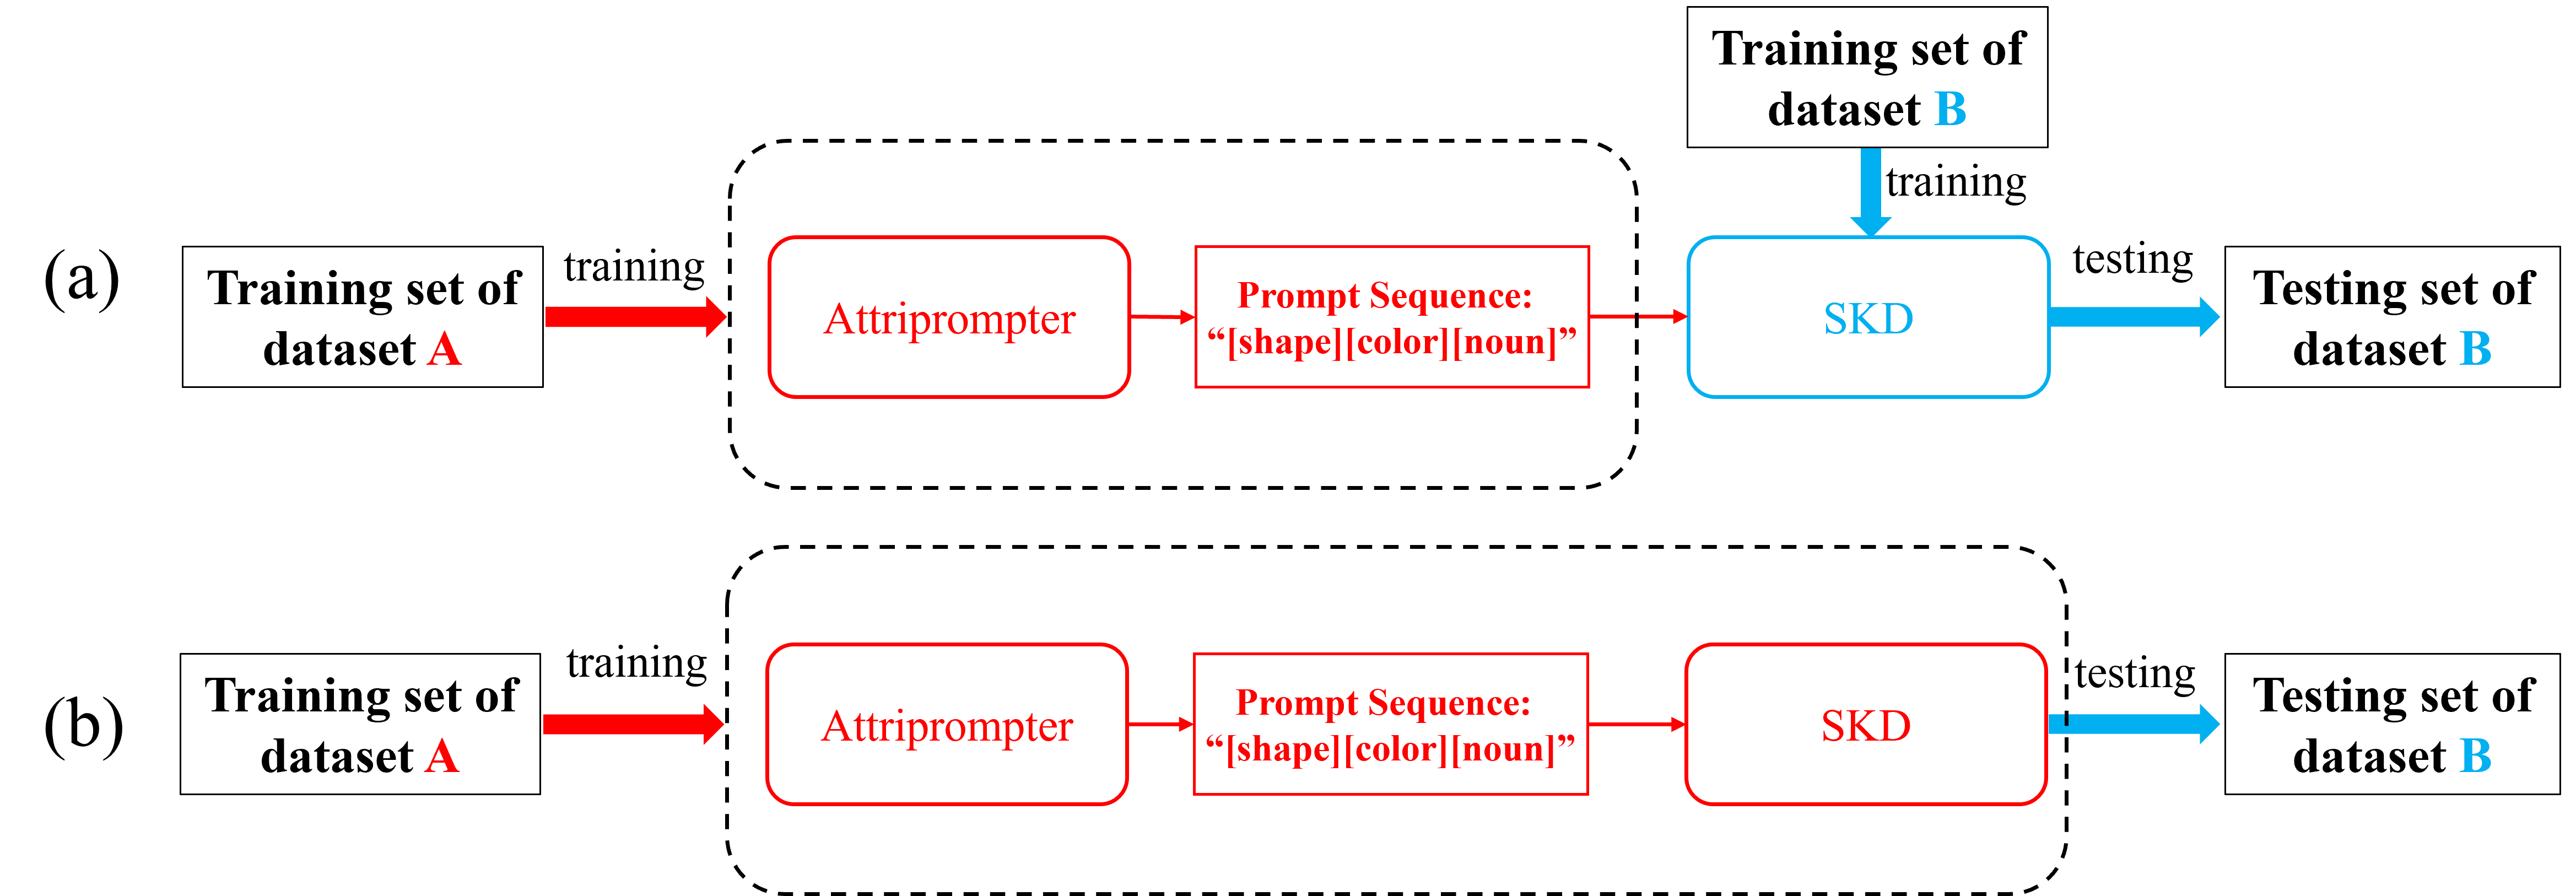
\includegraphics[width=\linewidth]{chapters/PAPERS/nucleiprompter__TMI_final_version/xu5.png}
\caption{两组跨域实验示意图。(a) 验证 AttriPrompter 的跨域能力；(b) 验证完整系统的 domain shift 性能。数据集 A 和数据集 B 分别表示源域和目标域。}
\label{fig:attrip_cross_domain}
\end{figure}

\subsection{AttriPrompter 的跨域能力}

表~\ref{tab:attrip_cross_capacity} 展示提示生成数据集和 SKD/测试数据集不同时的结果。使用 MoNuSeg 生成提示并在 MoNuSeg 上测试时，mAP 为 0.425；使用 CoNSeP 生成提示、在 MoNuSeg 上进行 SKD 和测试时，mAP 降至 0.405。反方向的结果也呈现类似趋势。说明提示属性具有一定的跨域迁移能力，但不同数据集在染色颜色和细胞核形态上的差异仍会造成性能下降。

\begin{table}[t]
\caption{AttriPrompter 跨域能力验证。}
\label{tab:attrip_cross_capacity}
\begin{center}
\resizebox{0.9\columnwidth}{!}{
\begin{tabular}{cccccc}
\toprule[1.5pt]
\textbf{用于生成提示的数据集} & \textbf{用于 SKD 和测试的数据集} & \textbf{mAP} & \textbf{AP50} & \textbf{AP75} & \textbf{AR} \\ \midrule[1.2pt]
\textbf{MoNuSeg} & \textbf{MoNuSeg} & 0.425 & 0.819 & 0.401 & 0.511 \\
\textbf{CoNSeP} & \textbf{MoNuSeg} & 0.405 & 0.759 & 0.400 & 0.480 \\ \midrule
\textbf{CoNSeP} & \textbf{CoNSeP} & 0.367 & 0.669 & 0.376 & 0.488 \\
\textbf{MoNuSeg} & \textbf{CoNSeP} & 0.339 & 0.669 & 0.324 & 0.441 \\ \bottomrule[1.5pt]
\end{tabular}
}
\end{center}
\vskip -0.15in
\end{table}

该结果表明，AttriPrompter 生成的属性并非只对单个数据集有效。即使提示生成域与测试域不同，常见的形状和颜色词仍然能够保留一定的检测能力；但若希望获得最佳性能，提示生成所依据的无标注图像应尽量接近目标测试域。

\subsection{完整系统的 domain shift}

第二组实验在源域上生成提示并完成 SKD，然后在不同目标域上测试。表~\ref{tab:attrip_domain_shift} 中的 ``MoNuSeg $\rightarrow$ CoNSeP'' 表示源域为 MoNuSeg、目标域为 CoNSeP；反向箭头表示相反方向。标准零样本方法不进行跨域训练，使用面向目标域手工设计的提示，作为灰色背景基线。

\begin{table}[t]
\caption{完整框架的 domain shift 实验。箭头表示源域到目标域的方向；标准零样本方法不执行跨域过程。最优结果以粗体表示。}
\label{tab:attrip_domain_shift}
\begin{center}
\resizebox{0.96\columnwidth}{!}{
\begin{tabular}{ccccccccc}
\toprule[1.5pt]
 & \multicolumn{4}{c}{\textbf{MoNuSeg $\rightarrow$ CoNSeP}} & \multicolumn{4}{c}{\textbf{CoNSeP $\rightarrow$ MoNuSeg}} \\ \cmidrule(r){2-5} \cmidrule(r){6-9}
\multirow{-2}{*}{\textbf{方法}} & \textbf{mAP} & \textbf{AP50} & \textbf{AP75} & \textbf{AR} & \textbf{mAP} & \textbf{AP50} & \textbf{AP75} & \textbf{AR} \\ \midrule
\rowcolor{lightgray}
\textbf{标准零样本（人工提示）} & 0.062 & 0.131 & 0.055 & 0.111 & 0.151 & 0.259 & 0.166 & 0.210 \\
\textbf{SSNS (2020)\cite{sahasrabudhe2020self}} & 0.122 & 0.310 & 0.101 & 0.274 & 0.111 & 0.204 & 0.115 & 0.169 \\
\textbf{VL-PLM (2022)\cite{zhao2022exploiting}} & 0.118 & 0.307 & 0.097 & 0.275 & 0.096 & 0.175 & 0.108 & 0.133 \\
\textbf{VLPM-NuD (2023)\cite{wu2023zeroshot}} & 0.152 & 0.389 & 0.080 & 0.257 & 0.173 & 0.250 & 0.171 & 0.225 \\
\textbf{AttriPrompter} & 0.082 & 0.182 & 0.061 & 0.124 & 0.168 & 0.287 & 0.175 & 0.199 \\
\textbf{AttriPrompter + SKD} & \textbf{0.178} & \textbf{0.439} & \textbf{0.112} & \textbf{0.285} & \textbf{0.260} & \textbf{0.594} & \textbf{0.178} & \textbf{0.356} \\ \bottomrule[1.5pt]
\end{tabular}
}
\end{center}
\end{table}

与同域结果相比，所有方法在 domain shift 下均出现不同程度的性能下降，但 AttriPrompter + SKD 仍取得最佳结果。源域提示在目标域中仍能发挥作用，可能是因为不同 H\&E 数据集之间具有一定共性，而自动生成过程倾向于选择自然语言中较常见的形状和颜色词。相反，人工提示容易加入 GLIP 预训练语料中覆盖不足的医学描述，因此在跨域条件下不一定更有效。SKD 在跨域场景中的收益说明，学生网络不仅能够修正初始检测框，还能通过源域伪标签学习较稳定的目标级结构表示。

\section{讨论与局限性}

本章实验说明，视觉语言模型应用于医学图像时，提示并非简单的类别名称替换。对于细胞核这类密集、相似且尺度较小的目标，形状和颜色属性提供了比医学名词更直接的视觉线索；程度增强可以扩大细粒度描述空间；相关性排序则利用了 GLIP 对输入序列顺序的敏感性。三者共同构成了从目标域图像到文本提示的自动化桥梁。

同时，SKD 解决的是“如何利用初始提示结果继续改善检测”的问题，而不是替代提示生成。伪标签实验表明，如果初始伪标签缺乏准确的目标语义，单纯增加自训练轮次并不能保证得到理想结果。知识蒸馏损失能够帮助学生网络保留 GLIP 的目标级知识，但最终结果仍受初始伪标签质量、学生网络结构和训练轮次影响。

本章仍存在以下局限。第一，当前属性生成主要关注形状和颜色，尚未充分利用纹理、染色强度、细胞核内部结构和空间上下文等信息。第二，SKD 需要多轮学生网络训练，计算开销较高，在大规模全视野图像上仍需要进一步优化。第三，domain shift 实验显示，提示和伪标签在跨域时会出现性能下降，说明当前方法还不能完全消除不同中心、设备和染色流程带来的域差异。后续研究可以从更丰富的属性生成、低成本的伪标签更新以及面向病理图像的域泛化策略三个方向继续改进。

\section{本章小结}

本章研究了结合自动属性提示和自训练知识蒸馏的无标注零样本细胞核检测方法。首先，通过提示实证分析发现，细粒度语义和合理的提示顺序能够显著影响 GLIP 的零样本预测。随后提出 AttriPrompter，从无标注病理图像中自动生成形状和颜色属性，并通过同义增强、程度增强和相关性排序构造最终提示序列。针对密集细胞核造成的漏检、误检和目标重叠问题，进一步构建 SKD 框架，以 GLIP 为教师、检测专用网络为学生，通过特征蒸馏和多轮自训练优化预测结果。

在 MoNuSeg 和 CoNSeP 上的实验表明，AttriPrompter 在无监督方法中取得了较好的综合性能；组件消融验证了程度增强和相关性排序的作用；伪标签和知识蒸馏实验说明，初始提示质量与 GLIP 先验知识迁移是性能提升的关键；不同学生网络和跨域实验则证明了该框架具有一定的结构泛化和域迁移能力。本章为后续章节进一步研究视觉文本化提示和跨域医学图像分析提供了基础。
